\chapter{Client}

\section{La communication client-serveur}

\paragraph{}
L’interface affichera les informations de la base de données (les exemples, ou les couples imagettes - transcriptions) et les modifiera. Pour ce faire, elle sera reliée au connecteur central via sa ressource REST. Le connecteur traitera les demandes de l’IHM et les enverra au connecteur de la base de données. Celui-ci exécutera les ordres de l’utilisateur sur la base et renverra les imagettes et les transcriptions au connecteur central qui les fera suivre à l’IHM. Les modifications (ajout ou modification d’une transcription ou suppression d’un exemple) seront enregistrées localement puis envoyées à la base de données lors du changement de page et du chargement d'une nouvelle page.
\newline{}
Les communications entre le client et le serveur se feront via des appels à une API \texttt{REST} dont nous définissons les différentes requêtes dans la liste ci-dessous. Chaque composant du client nécessitant des requêtes \texttt{REST} différentes, la liste est donc organisée par composant et l'organisation des appels sera détaillée par la suite.
\newline{}

\begin{description}[align=left]

\item [Général]

\item [GET] \texttt{/base/projectsAndDocuments}\newline{}
\begin{itshape}
Renvoie la liste des noms des projets, contenant pour chaque projet une liste des noms des documents qui le composent.
\end{itshape}

\item [POST] \texttt{/base/createNewProject/\{project\_name\}/\{list\_docs\}}\newline{}
\begin{itshape}
Crée un nouveau projet à partir du nom du projet et de la liste des noms des documents passée en paramètre.
\end{itshape}

\item [DELETE] \texttt{/base/deleteDocument/\{name\}}\newline{}
\begin{itshape}
Supprime le document de la base qui porte le nom donné, ainsi que son contenu.
\end{itshape}

\item [GET] \texttt{/base/availableRecognisers}\newline{}
\begin{itshape}
Renvoie la liste des noms des reconnaisseurs disponibles sur le serveur.
\end{itshape}

\item [POST] \texttt{/base/exportRecogniserExamples/\{name\}}\newline{}
\begin{itshape}
Récupère tous les exemples de la base qui sont contenus dans des projets utilisant le reconnaisseur dont le nom est passé en paramètre. Les exemples sont triés, ne sont retenus que ceux qui sont définis comme utilisables et validés. Ensuite, ces exemples sont exportés en tant que lot d'entraînement, vers le format d'entrée associé au reconnaisseur en question.
\end{itshape}

\newline{}
\item [Annotation / Validation]

\item [GET] \texttt{/base/documentPages/\{name\}}\newline{}
\begin{itshape}
Renvoie la liste des identifiants en base de données des pages qui composent un document dont le nom est donné en paramètre.
\end{itshape}

\item [GET] \texttt{/base/pageData/\{id\}}\newline{}
\begin{itshape}
Renvoie l'image associée à la page dont l'identifiant est donné en paramètre, ainsi que la liste des imagettes et des transcriptions des exemples qui la composent.
\end{itshape}

\item [POST] \texttt{/base/saveExampleEdits}\newline{}
\begin{itshape}
Enregistre dans la base de données les modifications de transcriptions décrites par l'objet JSON associé à la requête.
\end{itshape}

\item [PUT] \texttt{/base/disableExample/\{id\}}\newline{}
\begin{itshape}
Rend l'exemple dont l'identifiant est donné en paramètre inutilisable, \textit{i.e.} l'utilisateur juge que l'image est trop parasitée ou que l'exemple n'est pas pertinent.
\end{itshape}

\item [PUT] \texttt{/base/enableExample/\{id\}}\newline{}
\begin{itshape}
Rend l'exemple dont l'identifiant est donné en paramètre utilisable (principalement utilisé pour annuler l'action décrite ci-dessus).
\end{itshape}

\item [POST] \texttt{/base/validateExamples}\newline{}
\begin{itshape}
Valide tous les exemples dont les identifiants sont fournis dans une liste JSON associée à la requête.
\end{itshape}

\newline{}
\item [Découpe]

\item [GET] \texttt{/base/documentPagesWithImages/\{name\}}\newline{}
\begin{itshape}
Renvoie la liste des identifiants et des images associés aux pages qui composent le document portant le nom donné.
\end{itshape}

\item [POST] \texttt{/base/addDocumentGroundtruth/\{name\}}\newline{}
\begin{itshape}
Ajoute à la base la vérité terrain donnée dans l'objet PiFF (donc JSON) associé à la requête, et l'associe au document dont le nom est donné en paramètre.
\end{itshape}

\item [GET] \texttt{/base/recogniseImages/\{name\}}\newline{}
\begin{itshape}
Envoie la liste des imagettes contenues dans le document donné au reconnaisseur associé au projet contenant ce document. La réponse à cette requête est une liste de transcriptions trouvées par le reconnaisseur.
\end{itshape}

\end{description}

%-------------------------------------------------------------------------------

\section{Les différents composants de l'interface}

\paragraph{}
\texttt{Angular} permet d'organiser les interfaces web par composants. Notre interface ne contiendra que des composants indépendants interagissant les uns avec les autres. Tous les composants seront regroupés dans le composant de \textit{routing} \texttt{app-root}.

\subsection{Première itération}

Pour la première itération, l’interface est réduite à sa forme la plus simple qui répond au cahier des charges, à savoir ouvrir un document de travail et valider ou invalider les transcriptions. L’IHM aura donc deux composants : la page d’accueil et la page de validation des annotations.

\paragraph{}
La page d’accueil permet à l’utilisateur de choisir le projet sur lequel il veut travailler, ainsi que d'en créer de nouveaux en choisissant les documents qui le composent. Pour afficher la liste des projets existants, le composant \texttt{accueil} appellera la requête \texttt{GET} \texttt{/base/projectsAndDocuments} et, pour créer un nouveau projet, il appellera \texttt{POST} \texttt{/base/createNewProject/\{project\_name\}/\{list\_docs\}}. L'utilisateur a également la possibilité de supprimer un document existant en faisant appel à la requête \texttt{DELETE} \texttt{/base/deleteDocument/\{name\}}.


\paragraph{}
La page de validation, comme son nom l’indique, permettra de valider ou d’invalider les transcriptions de la base de données relatives au document ouvert. Ces transcriptions ayant été réalisées par des humains, elles seront considérées comme vraies, et l’utilisateur pourrait les invalider seulement s’il manque des mots, ou si l’imagette est jugée peu pertinente pour l’apprentissage (par exemple, si le texte est presque illisible ou si l’imagette ne contient pas de texte du tout).
\newline{}
Pour ce faire, le composant \texttt{validation} réalisera différents appels à l'API \texttt{REST}. Toud d'abord, il faut pouvoir identifier quelles pages composent le document ouvert par l'utilisateur. Cela sera effectué par l'appel à la requête \texttt{GET} \texttt{/base/documentPages/\{name\}}. Pour obtenir la liste des imagettes et des transcriptions qui composent une page, le composant appellera \texttt{GET} \texttt{/base/pageData/\{id\}}. Lorsque l'utilisateur changera de page après avoir parcouru toutes les transcriptions d'une page, on réalisera un appel à la requête \texttt{POST} \texttt{/base/saveExampleEdits} afin d'enregistrer en base de données les modifications effectuées sur les transcriptions. De plus, un exemple peut être invalidé en appelant la requête \texttt{PUT} \texttt{/base/disableExample/\{id\}} ou au contraire redevenir valide après l'appel à la requête \texttt{PUT} \texttt{/base/enableExample/\{id\}}. Enfin, l'appel à \texttt{POST} \texttt{/base/validateExamples} permet de valider tous les exemples valides de la page.

%------------------------------------------------------------------------------

\newpage{}

\subsection{Deuxième itération}

Pour la deuxième itération, nous implémenterons les fonctionnalités supplémentaires décrites dans les rapports précédents.

\paragraph{}
Dans la page d'accueil, nous rajouterons la possibilité d'interagir avec un reconnaisseur d'écriture manuscrite. Pour cela, le composant appellera la requête \texttt{GET} \texttt{/base/availableRecognisers} afin d'obtenir la liste des noms des reconnaisseurs disponibles sur le serveur pour que l'utilisateur fasse son choix. De plus, l'appel à la requête \texttt{POST} \texttt{/base/exportRecogniserExamples/\{name\}} permettra de récupérer tous les exemples de la base contenus dans des projets utilisant le reconnaisseur dont le nom est passé en paramètre. Les exemples seront triés pour ne retenir que ceux définis comme utilisables et validés. Ensuite, ces exemples seront exportés en tant que lot d'entraînement, vers le format d'entrée associé au reconnaisseur en question.

\paragraph{}
Nous proposerons également une page de découpe des zones ou des paragraphes du document à l’aide d’outils graphiques. Pour ce faire, nous aurons besoin de récupérer l'image de la page scannée afin de la découper, ce qui sera effectué via l'appel à la requête \texttt{GET} \texttt{/base/documentPagesWithImages/\{name\}} qui renvoie la liste des identifiants et des images associés aux pages qui composent le document portant le nom \textit{name}. En outre, ce composant devra permettre d'ajouter dans la base de données la vérité-terrain générée dans cette page de l'IHM. Ceci sera effectué via la requête \texttt{POST} \texttt{/base/addDocumentGroundtruth/\{name\}}, \textit{name} étant le nom du document ouvert. Enfin, il avait été spécifié dans le précédent rapport que la page de découpe devra posséder un bouton permettant d'envoyer la liste des imagettes de la page découpée au reconnaisseur associé au projet contenant le document ouvert pour qu'il propose des transcriptions. Ainsi, un \textit{click} sur ce bouton fera appel à la requête \texttt{REST} \texttt{GET} \texttt{/base/recogniseImages/\{name\}}.

\paragraph{}
Lors de l’ouverture d’un nouveau document de travail, il devra être possible d’utiliser des manuscrits scannés qui ne possèdent pas de vérité terrain. L’utilisateur aura alors la possibilité d’annoter le manuscrit manuellement ou de le faire passer par un reconnaisseur d’écriture après avoir découpé les zones du manuscrit via la page de découpe de l’interface.

\paragraph{}
L’interface possèdera donc une page d’annotation manuelle ainsi qu'une page de visualisation et de correction des résultats de l'apprentissage du reconnaisseur. Les deux composants seront sensiblement les mêmes, à quelques différences près décrites dans le rapport de spécification.
\newline{}
Les appels \texttt{REST} effectués par ces composants seront les mêmes et seront identiques à ceux effectués par le composant de la page de validation, soit \texttt{GET} \texttt{/base/documentPages/\{name\}} pour obtenir les identifiants des pages composant le document ouvert, \texttt{GET} \texttt{/base/pageData/\{id\}} qui renvoie la liste des exemples qui composent une page, \texttt{POST} \texttt{/base/saveExampleEdits} afin d'enregistrer en base de données les modifications effectuées sur les transcriptions, ainsi que \texttt{PUT} \texttt{/base/disableExample/\{id\}} ou \texttt{PUT} \texttt{/base/enableExample/\{id\}} pour cacher ou réhabiliter un exemple. Enfin, on pourra valider tous les exemples valides grâce à la requête \texttt{POST} \texttt{/base/validateExamples}.

\paragraph{}
Enfin, la dernière page de l’interface de la deuxième itération sera la page de validation qui a déjà été réalisée lors du premier rendu. Deux modifications y seront apportées pour la deuxième itération.
\newline{}
Tout d'abord, une fenêtre sera ajoutée pour visualiser la page courante en miniature, avec ses zones de découpe affichées par dessus, ainsi qu’un rectangle montrant la position courante de l’utilisateur, afin que ce dernier ait constamment accès à sa position dans le document. Nous obtiendrons l'image de la page entière grâce à la requête \texttt{GET} \texttt{/base/pageData/\{id\}}.
\newline{}
Ensuite, la bannière en haut de la page affichera si les transcriptions ont été réalisées manuellement par un humain ou par le reconnaisseur d'écriture, car l'attention fournie par l'utilisateur devrait être moindre pour un manuscrit annoté manuellement où les fautes sont théoriquement moins nombreuses. Savoir si la transcription a été faite manuellement ou par le reconnaisseur permettrait d'augmenter la rapidité de la validation finale. Cette information sera également obtenue grâce à l'appel \texttt{REST} précédent.

\paragraph{}
En résumé, à la fin de la deuxième itération, nous aurons cinq composants différents : la page d’accueil, la page de découpe des zones du document, la page d’annotation manuelle, la page de visualisation de la reconnaissance et la page de validation finale des transcriptions.

%-------------------------------------------------------------------------------
\section{Interactions entre les différents composants de l'interface}

\paragraph{}
L’utilisateur peut naviguer entre les différents composants via les boutons de l’interface.
\newline{}
Tout d’abord, une icône permettant de revenir à la page d’accueil sera présente en haut à gauche de chaque page - à l’exception de la page d’accueil. Sur cette dernière, le choix du document ouvre celui-ci dans la page de l’interface qui lui correspond, soit :

\begin{itemize}
\item la page de découpe si aucun travail n’a été réalisé au préalable sur ce document ;
\item la page d’annotation manuelle si les découpes ont déjà été réalisées et que l’utilisateur n’a pas exporté le document vers le reconnaisseur ;
\item la page de visualisation des transcriptions du reconnaisseur si une reconnaissance a été réalisée sur le document ;
\item ou la page de validation finale si toutes les transcriptions ont déjà été renseignées.
\end{itemize}

Des boutons de navigation dans les différentes pages sont également présents sur certaines pages, comme décrit dans la partie précédente. Les interactions sont visibles dans le schéma ci-dessous :

\begin{mdframed}[frametitle={Figure 7 : Schéma des interactions entre les différents composants de l'IHM}, innerbottommargin=10]
\begin{center}
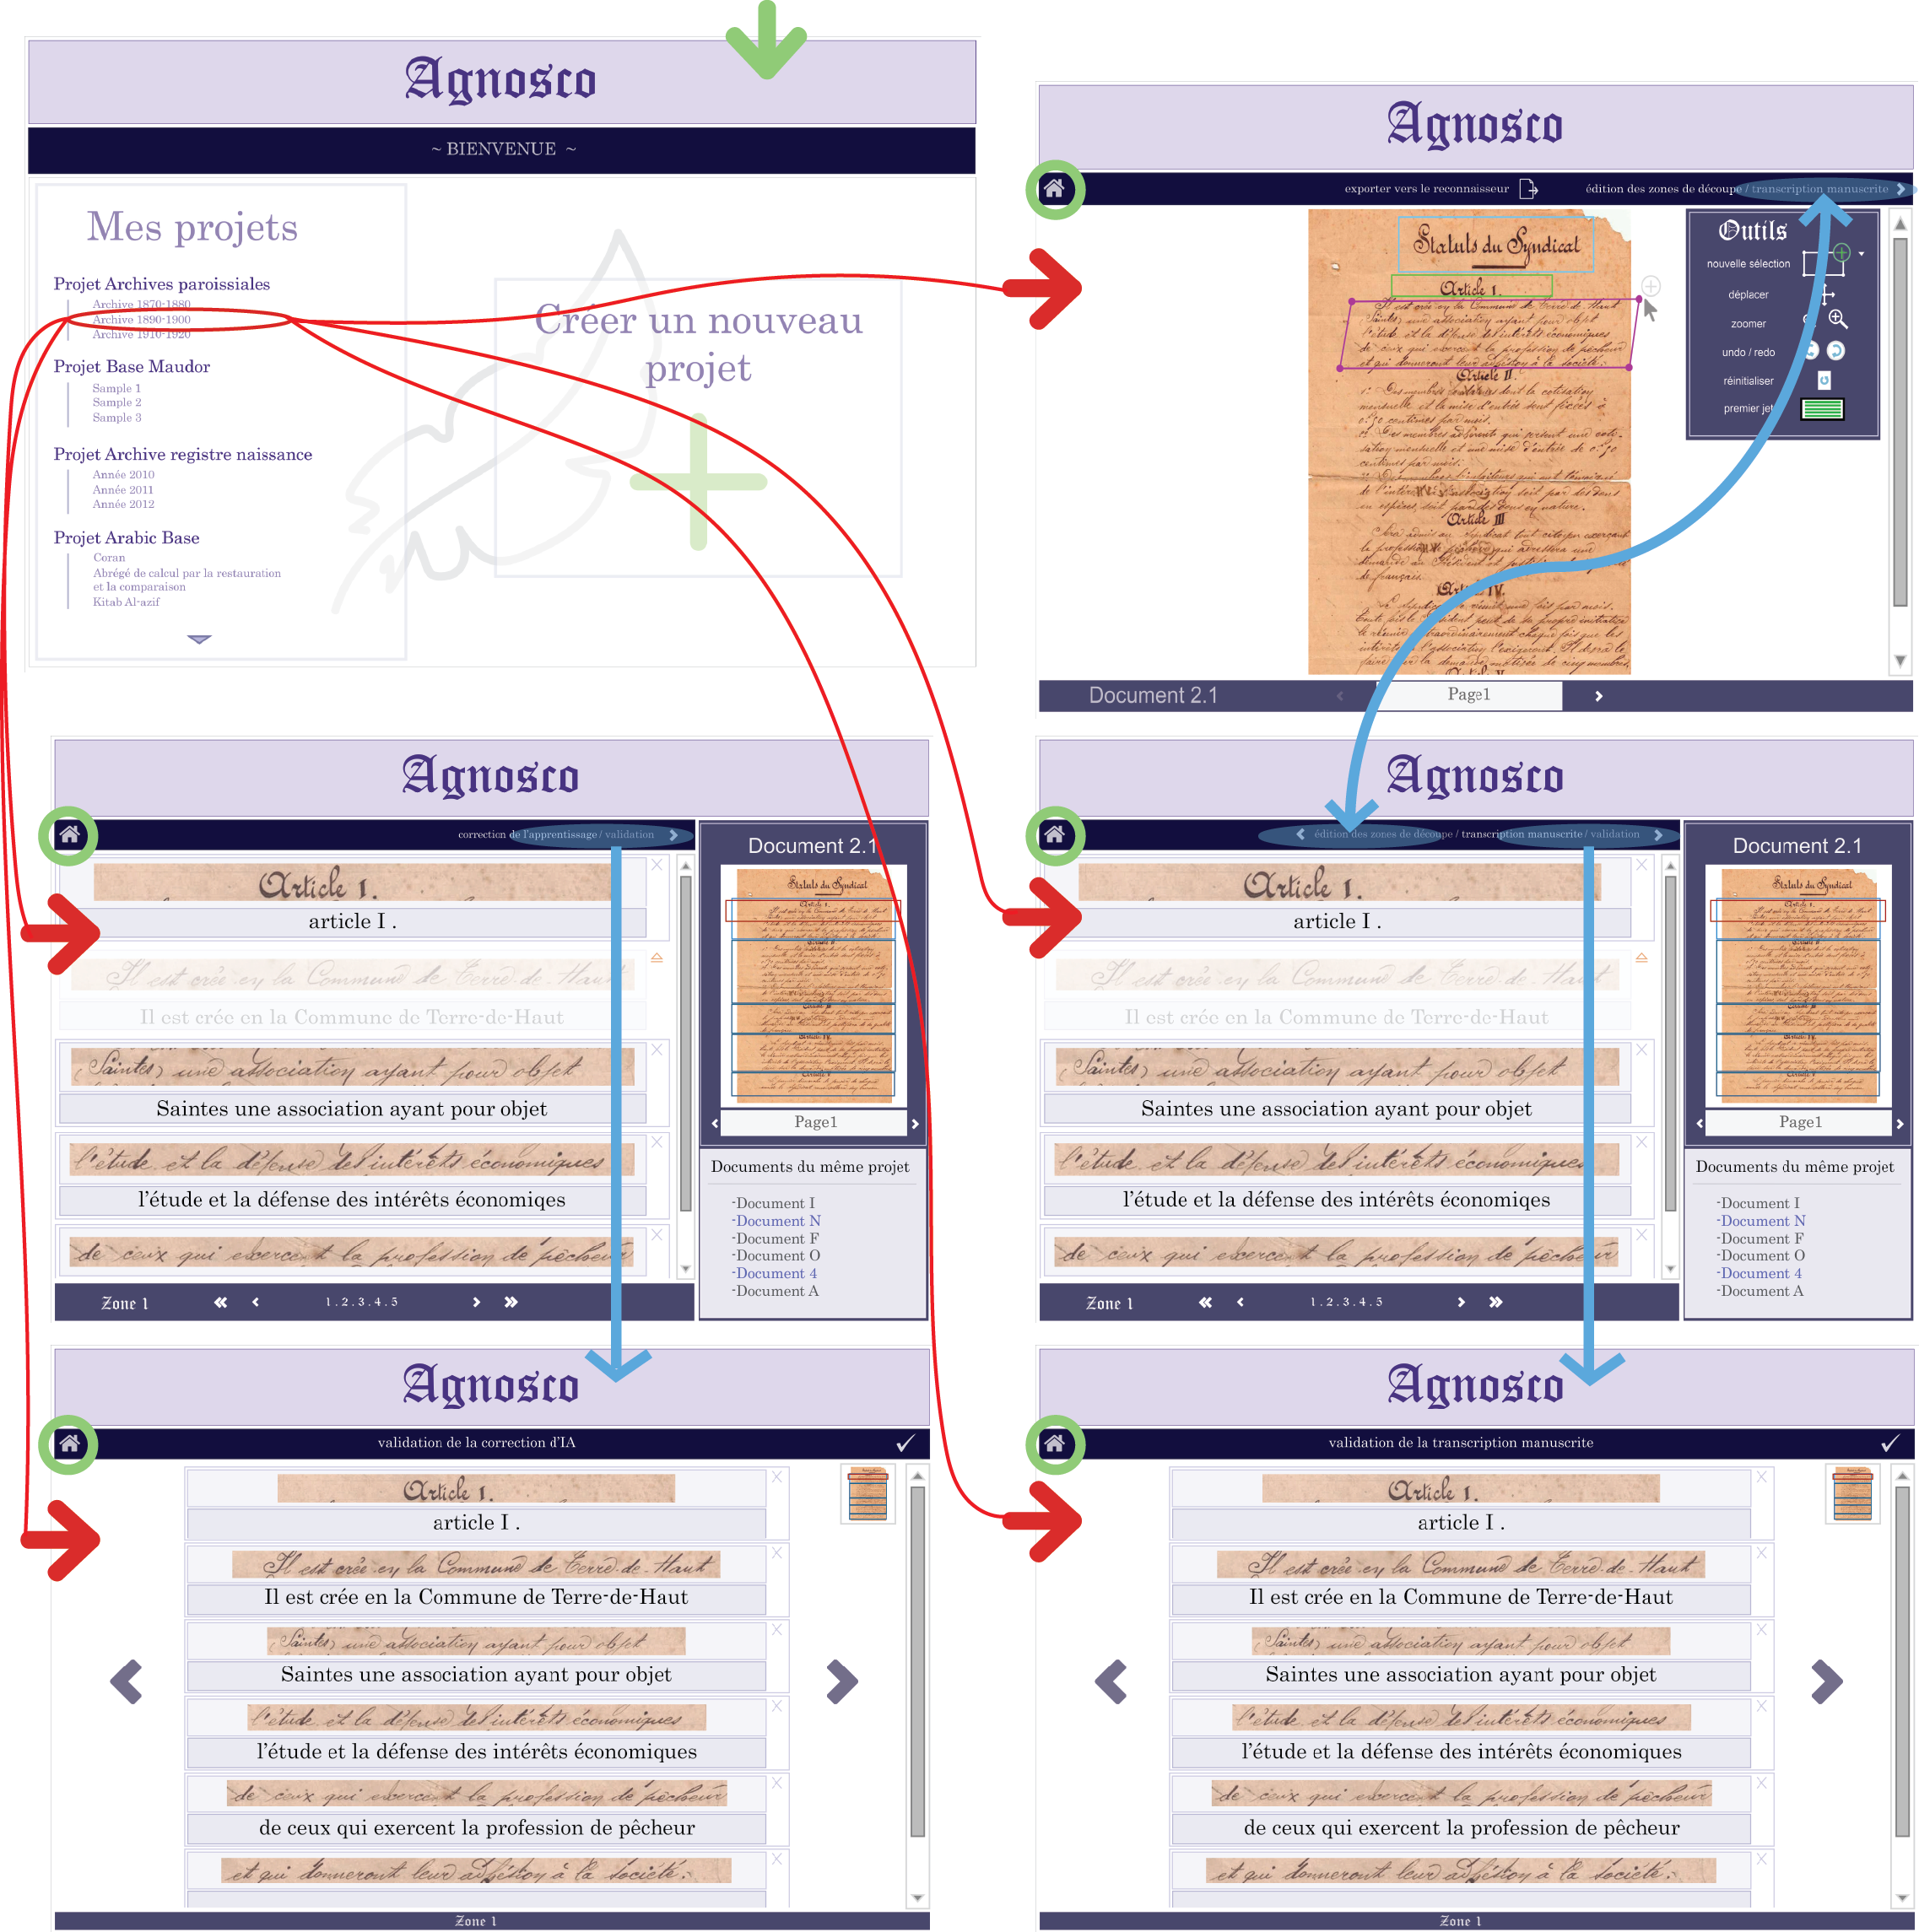
\includegraphics[scale=0.5]{assets/schemaIHMinteractions.png}
\end{center}
\end{mdframed}




\newpage{}
\begin{mdframed}[frametitle={Figure 1 : Maquette de la page d'accueil de l'IHM}, innerbottommargin=10]
\begin{center}
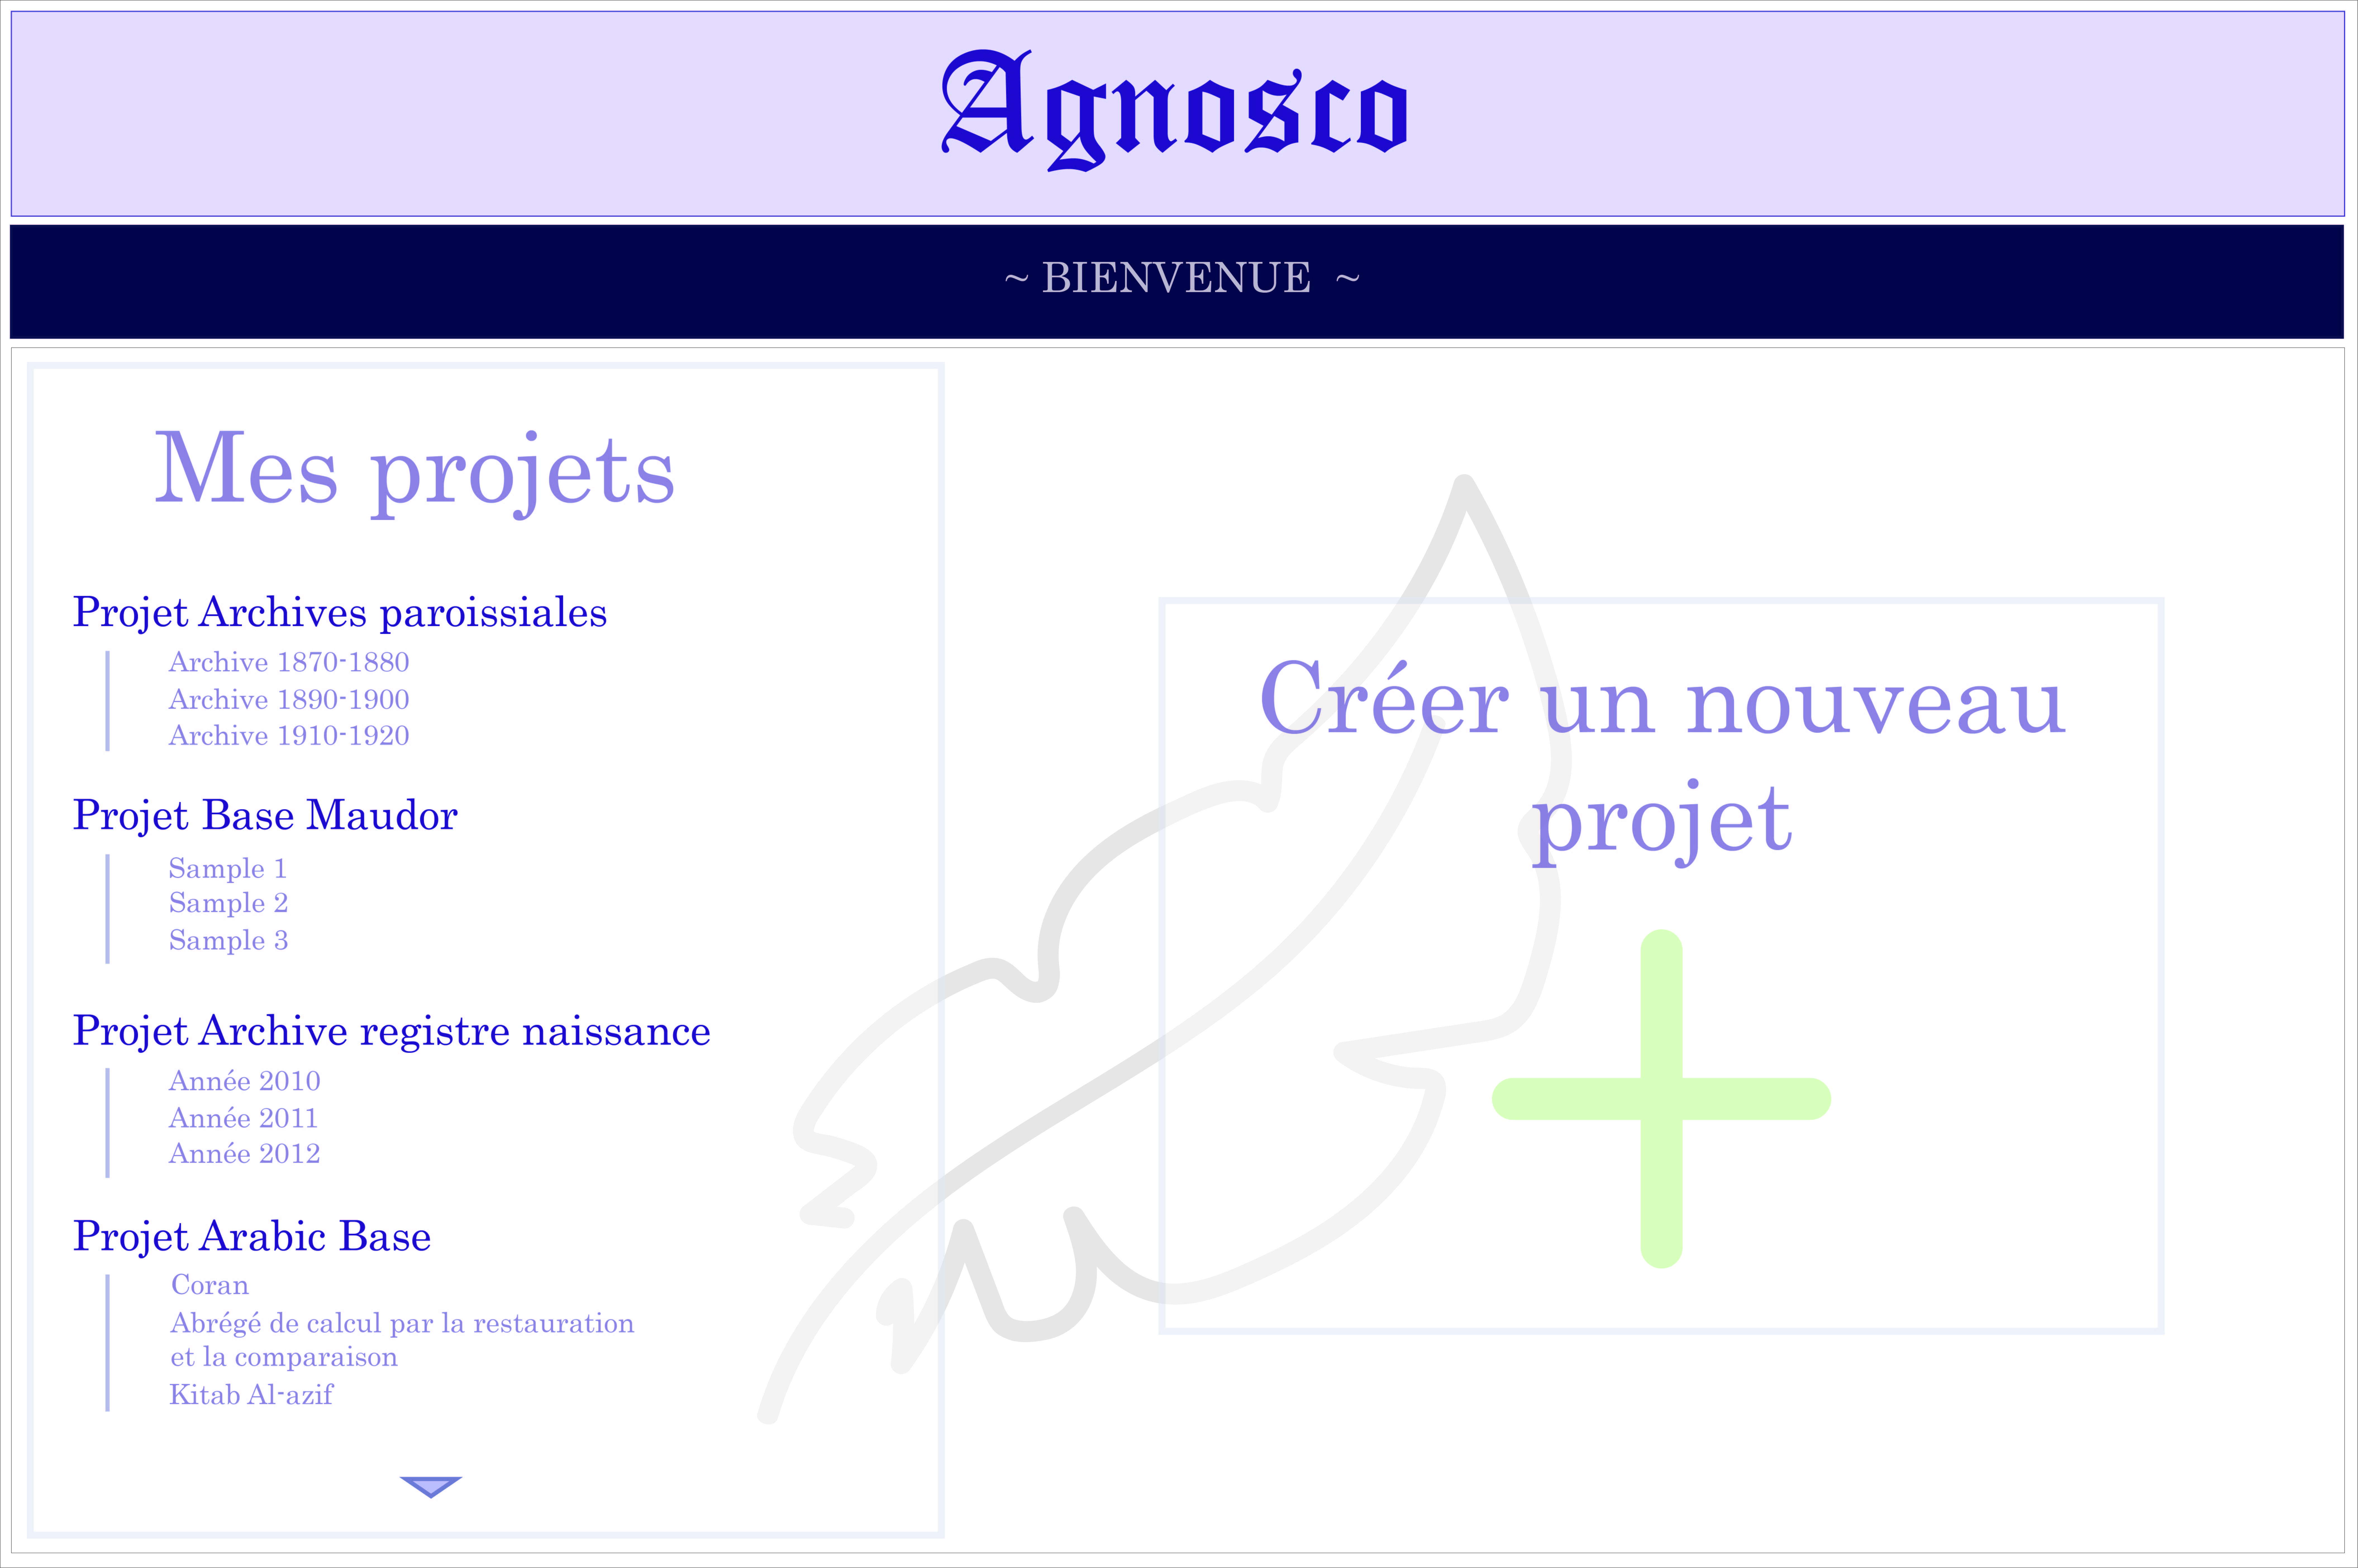
\includegraphics[scale=0.04]{assets/maquetteIHMaccueil.jpg}
\end{center}
\end{mdframed}


\begin{mdframed}[frametitle={Figure 2 : Maquette de la page de validation des annotations}, innerbottommargin=10]
\begin{center}
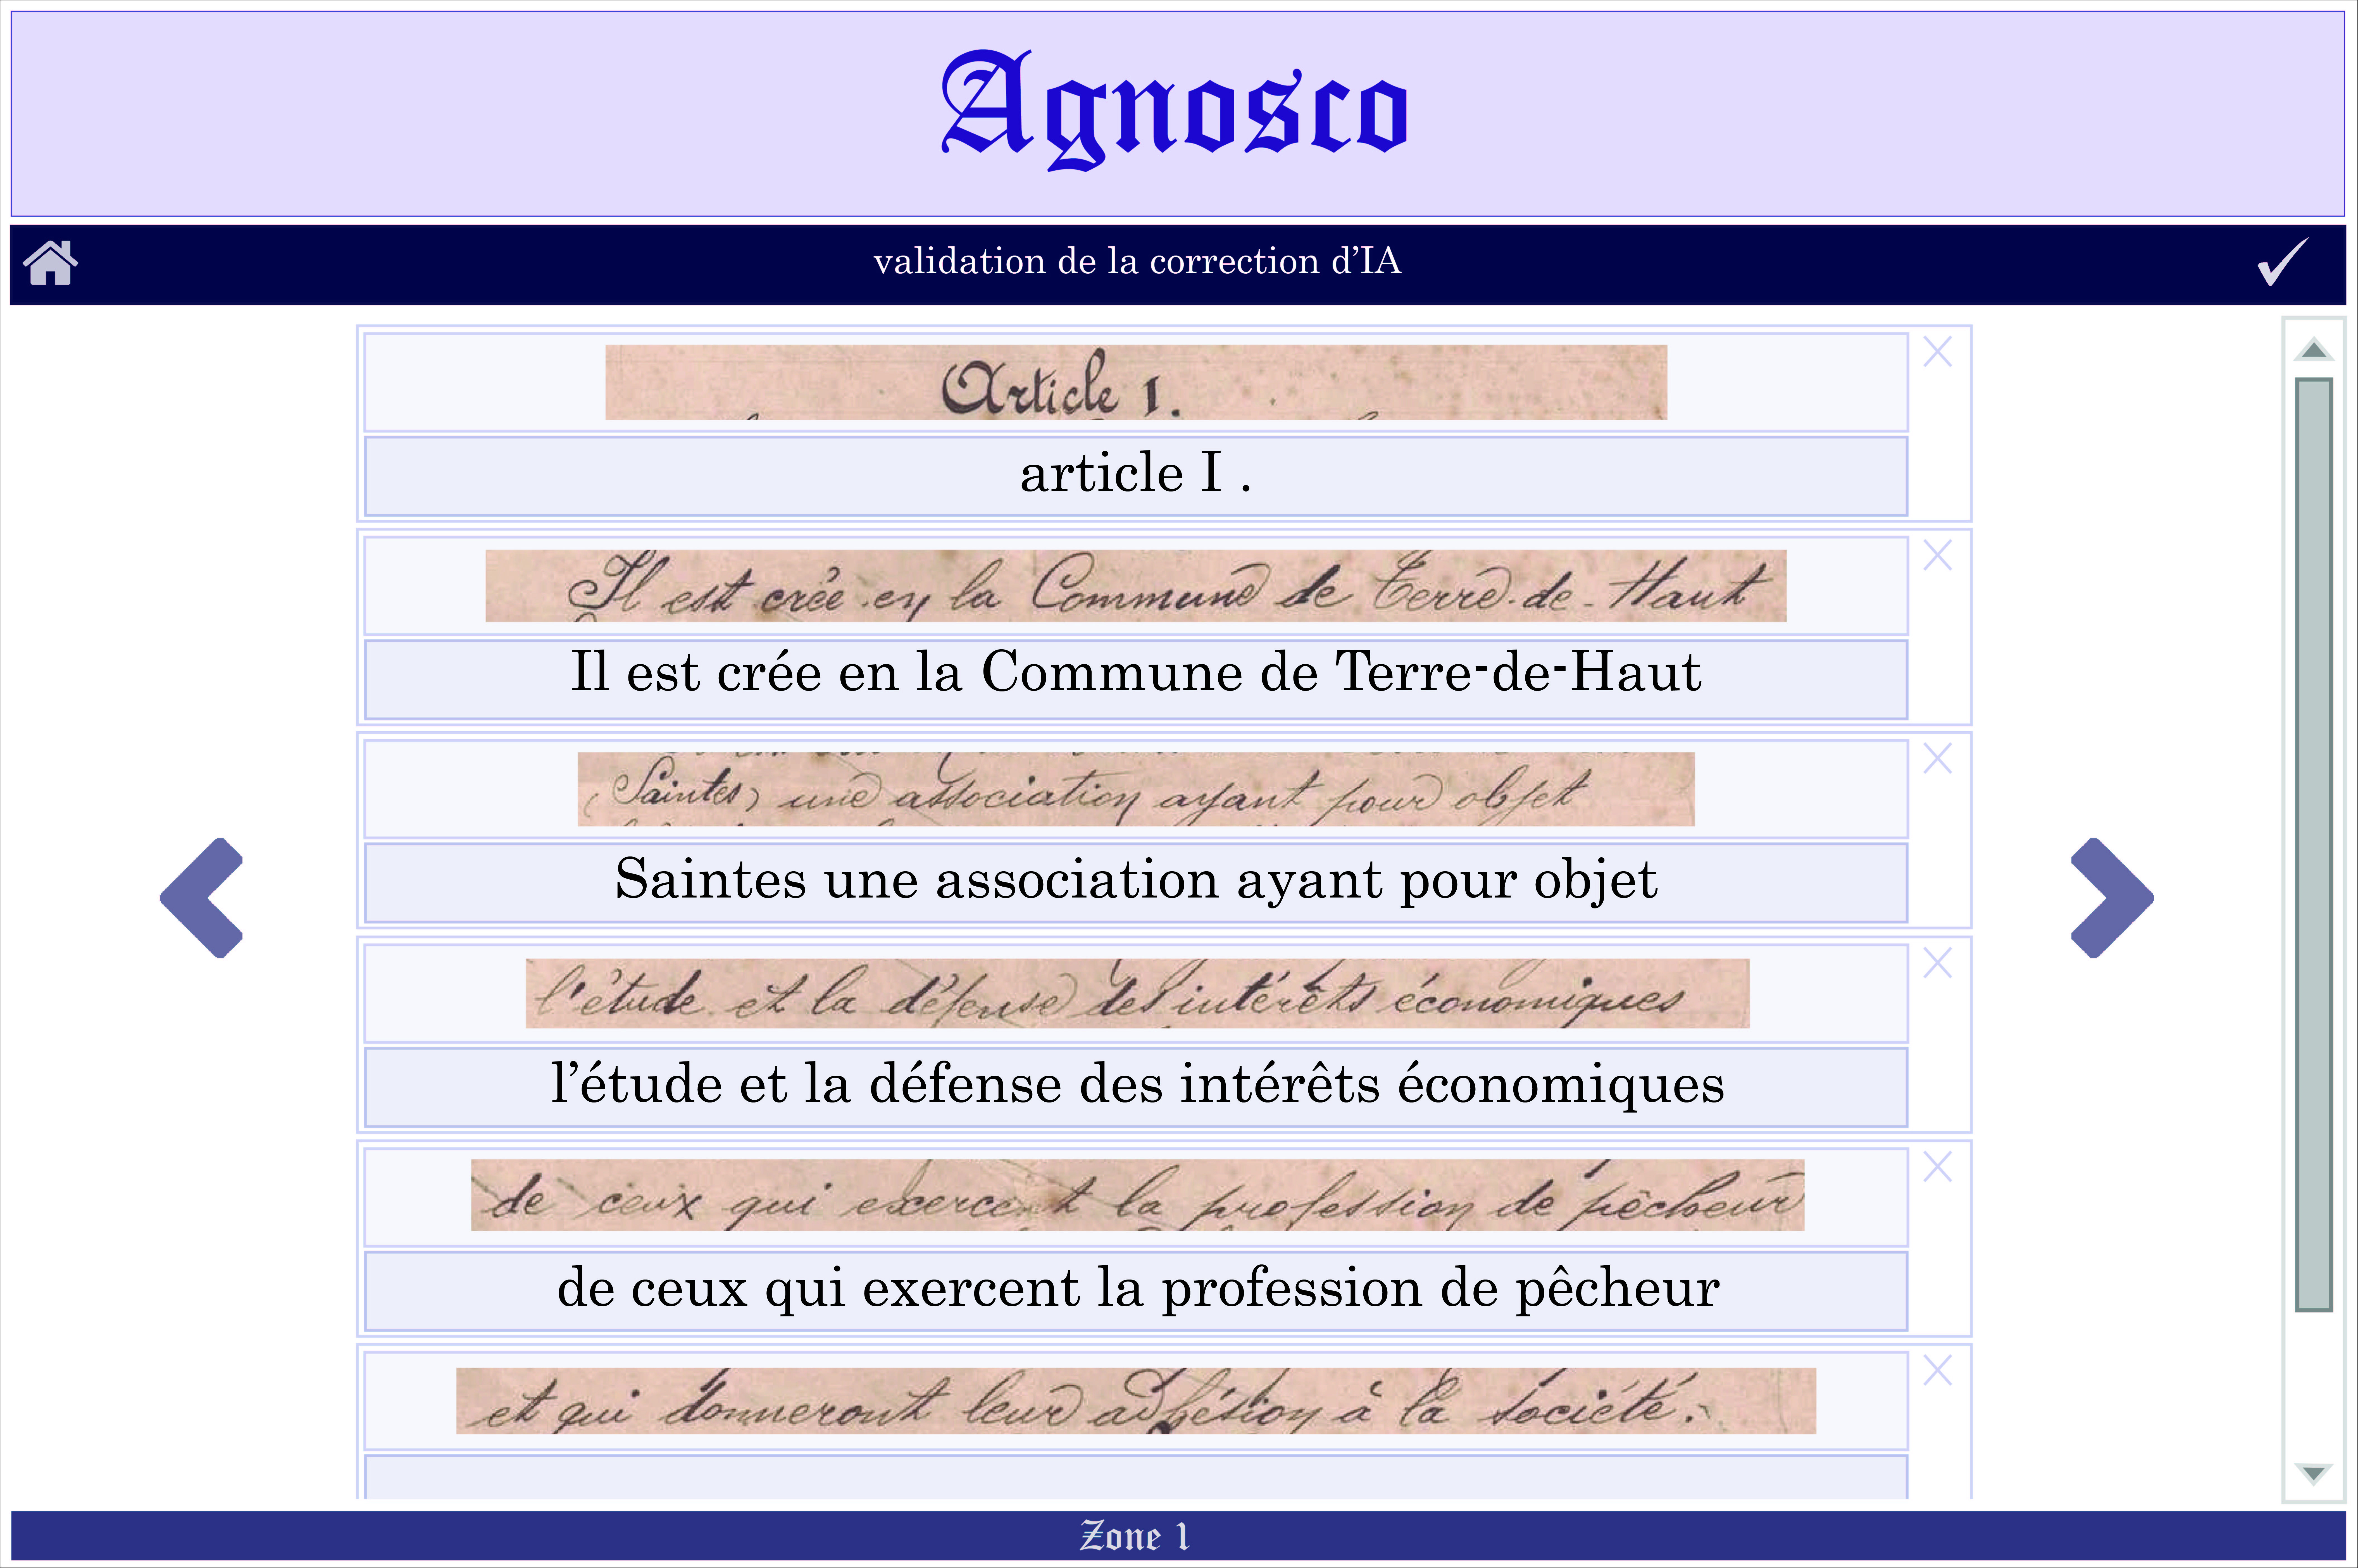
\includegraphics[scale=0.04]{assets/maquetteIHMvalidation1.jpg}
\end{center}
\end{mdframed}


\begin{mdframed}[frametitle={Figure 3 : Maquette de la page de découpe des zones}, innerbottommargin=10]
\begin{center}
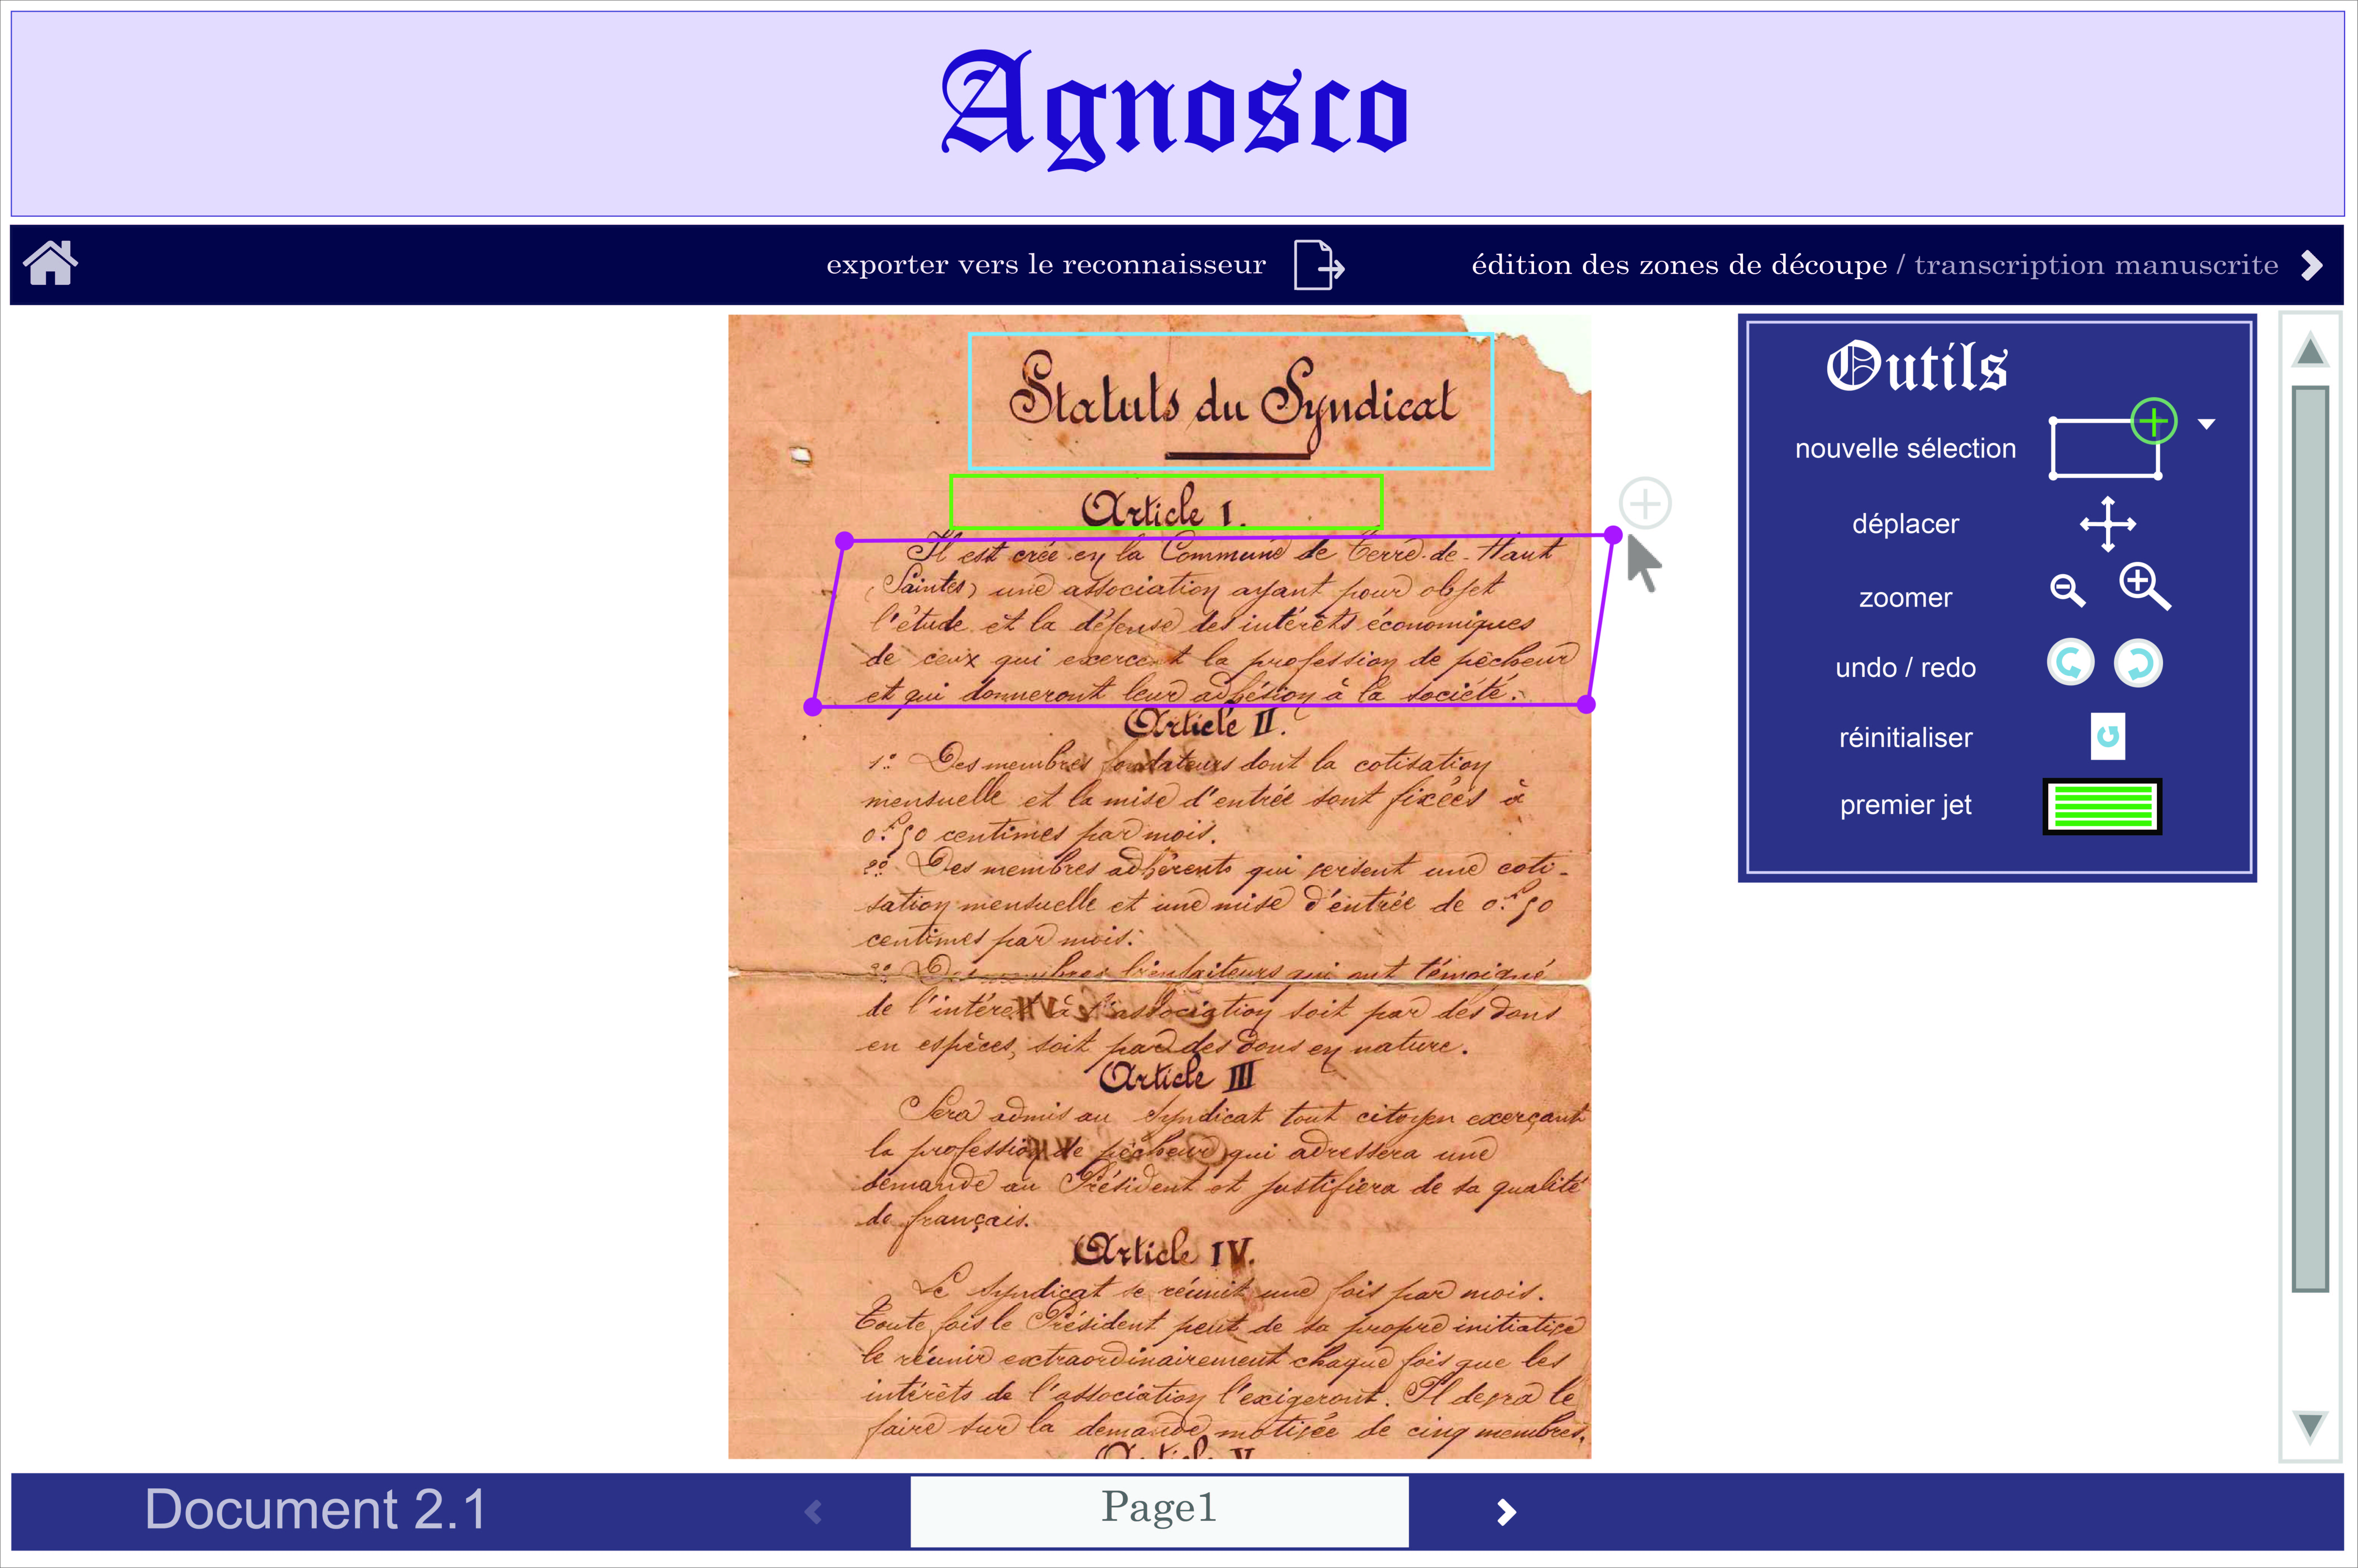
\includegraphics[scale=0.04]{assets/maquetteIHMdecoupes.jpg}
\end{center}
\end{mdframed}


\begin{mdframed}[frametitle={Figure 4 : Maquette de la page d'annotation manuelle}, innerbottommargin=10]
\begin{center}
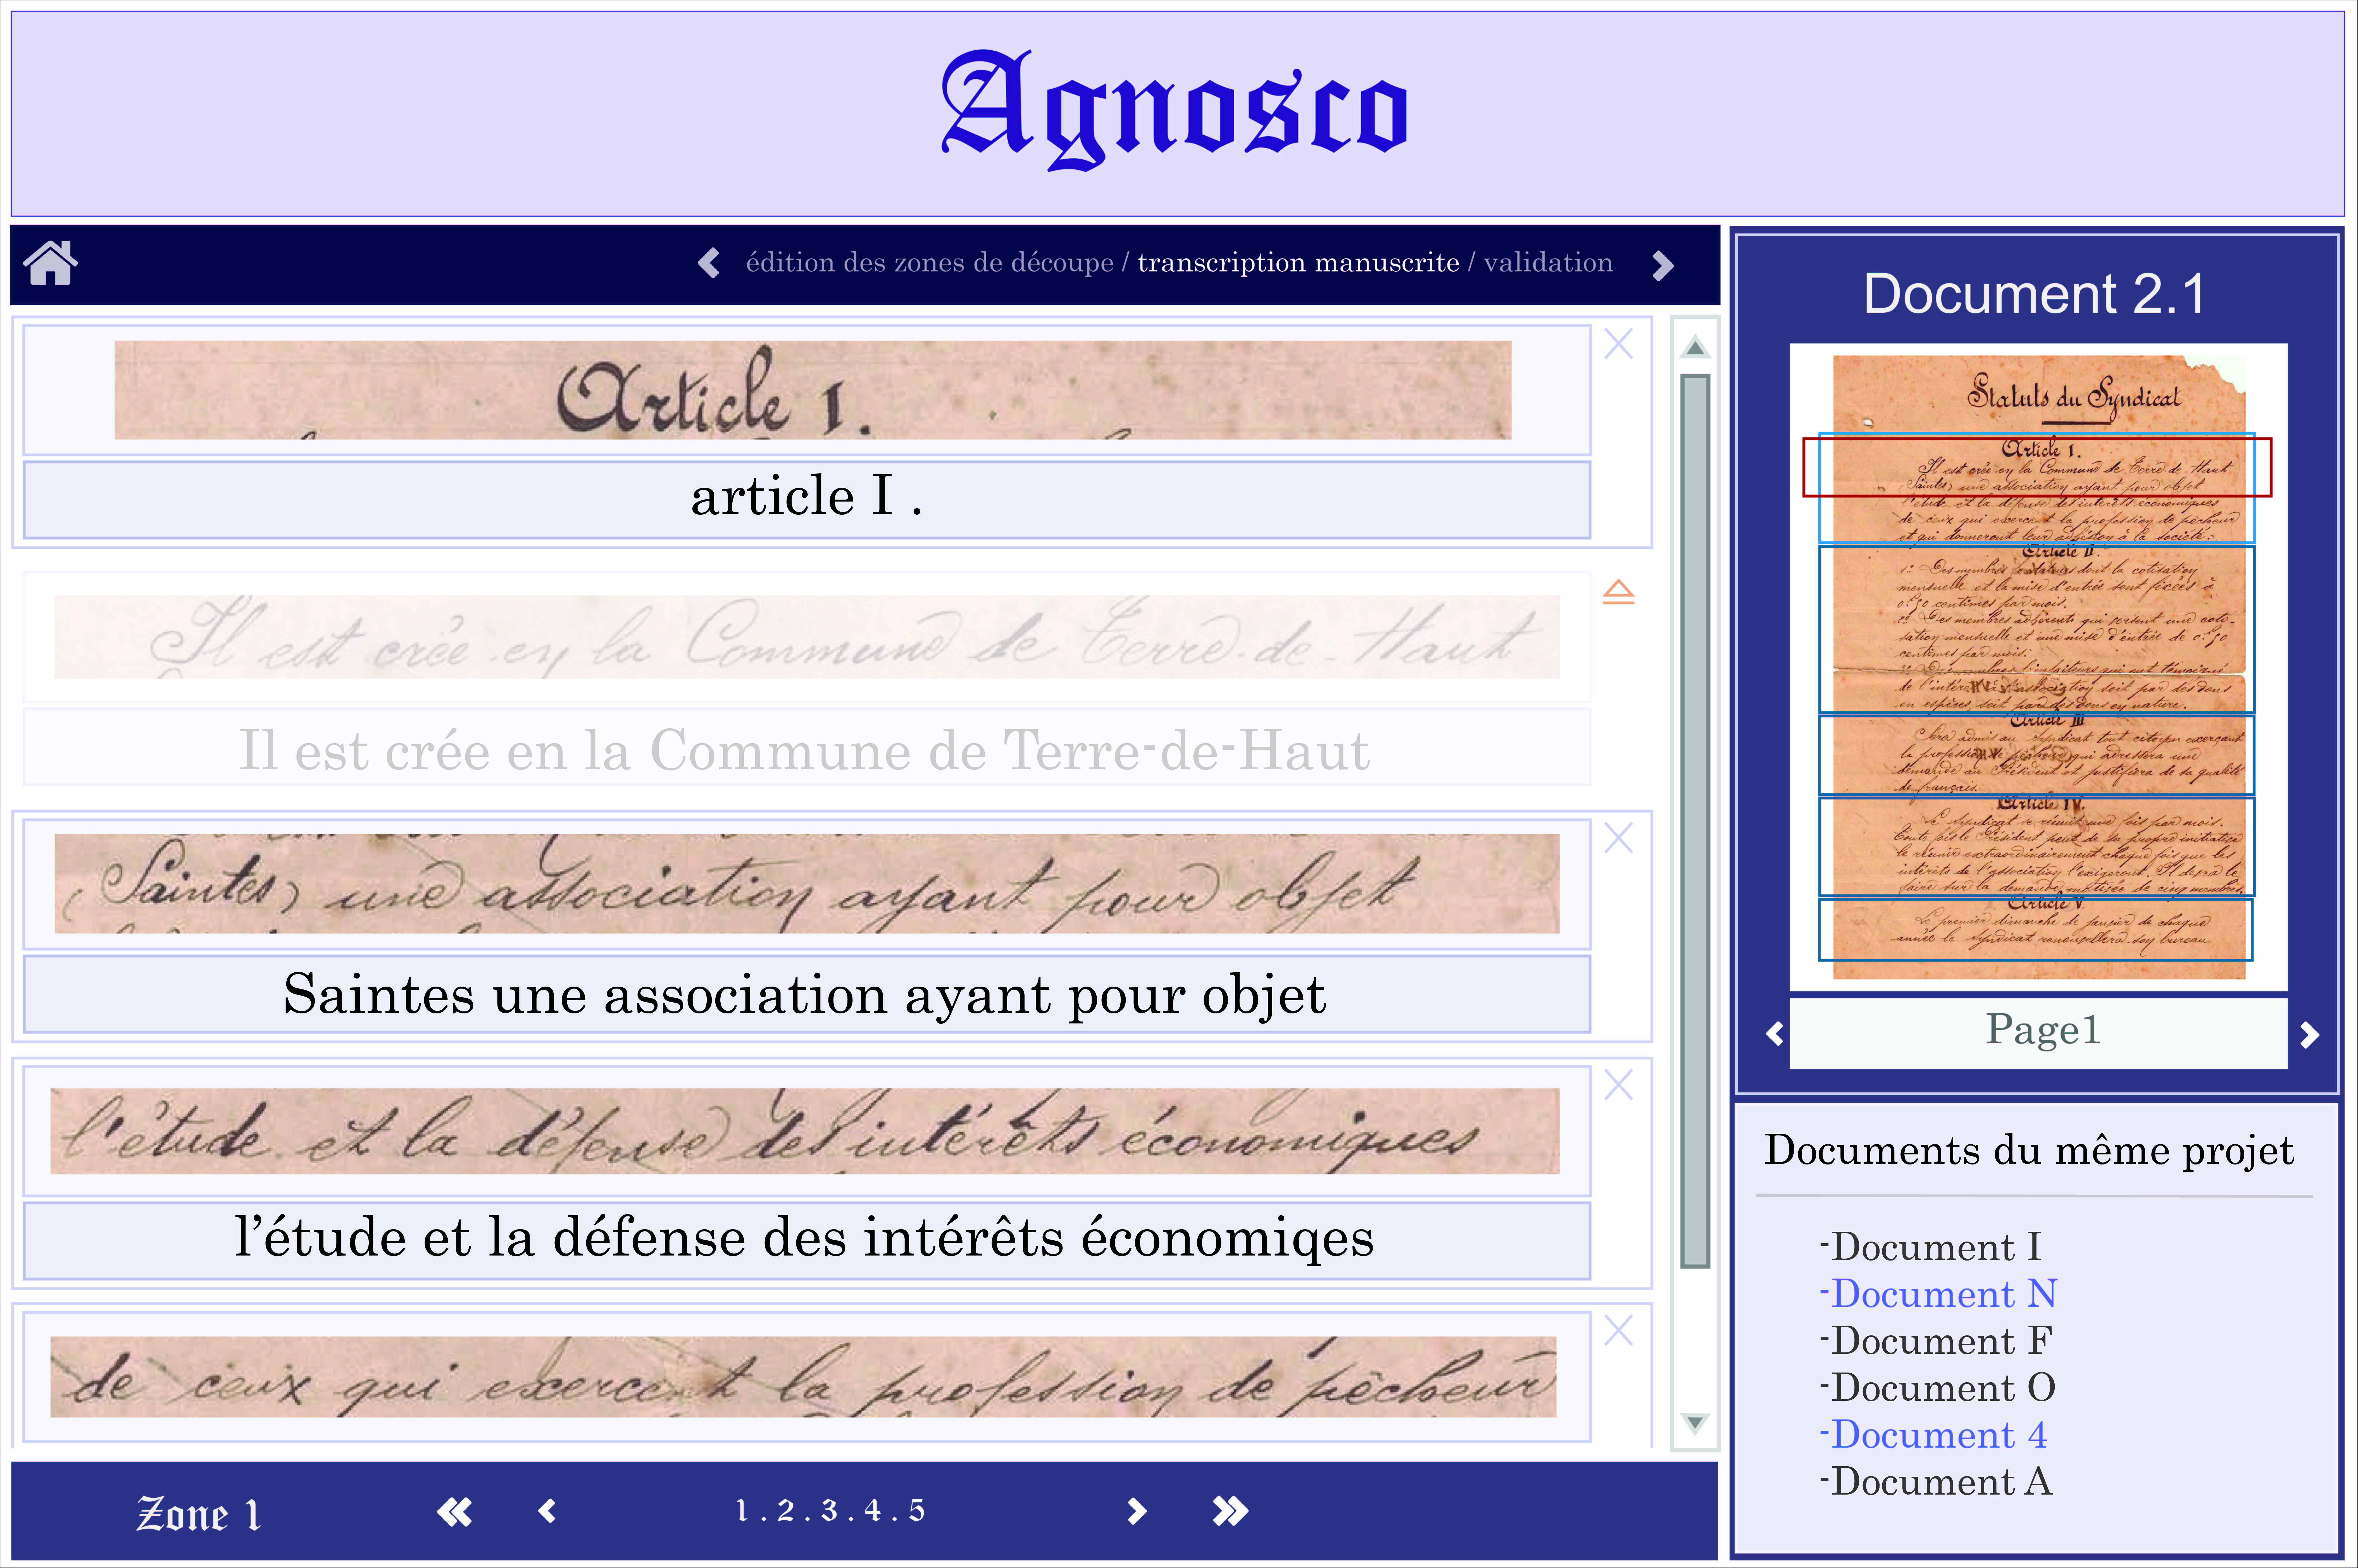
\includegraphics[scale=0.04]{assets/maquetteIHMtranscriptionmanu.jpg}
\end{center}
\end{mdframed}


\begin{mdframed}[frametitle={Figure 5 : Maquette de la page de visualisation des transcriptions du reconnaisseur}, innerbottommargin=10]
\begin{center}
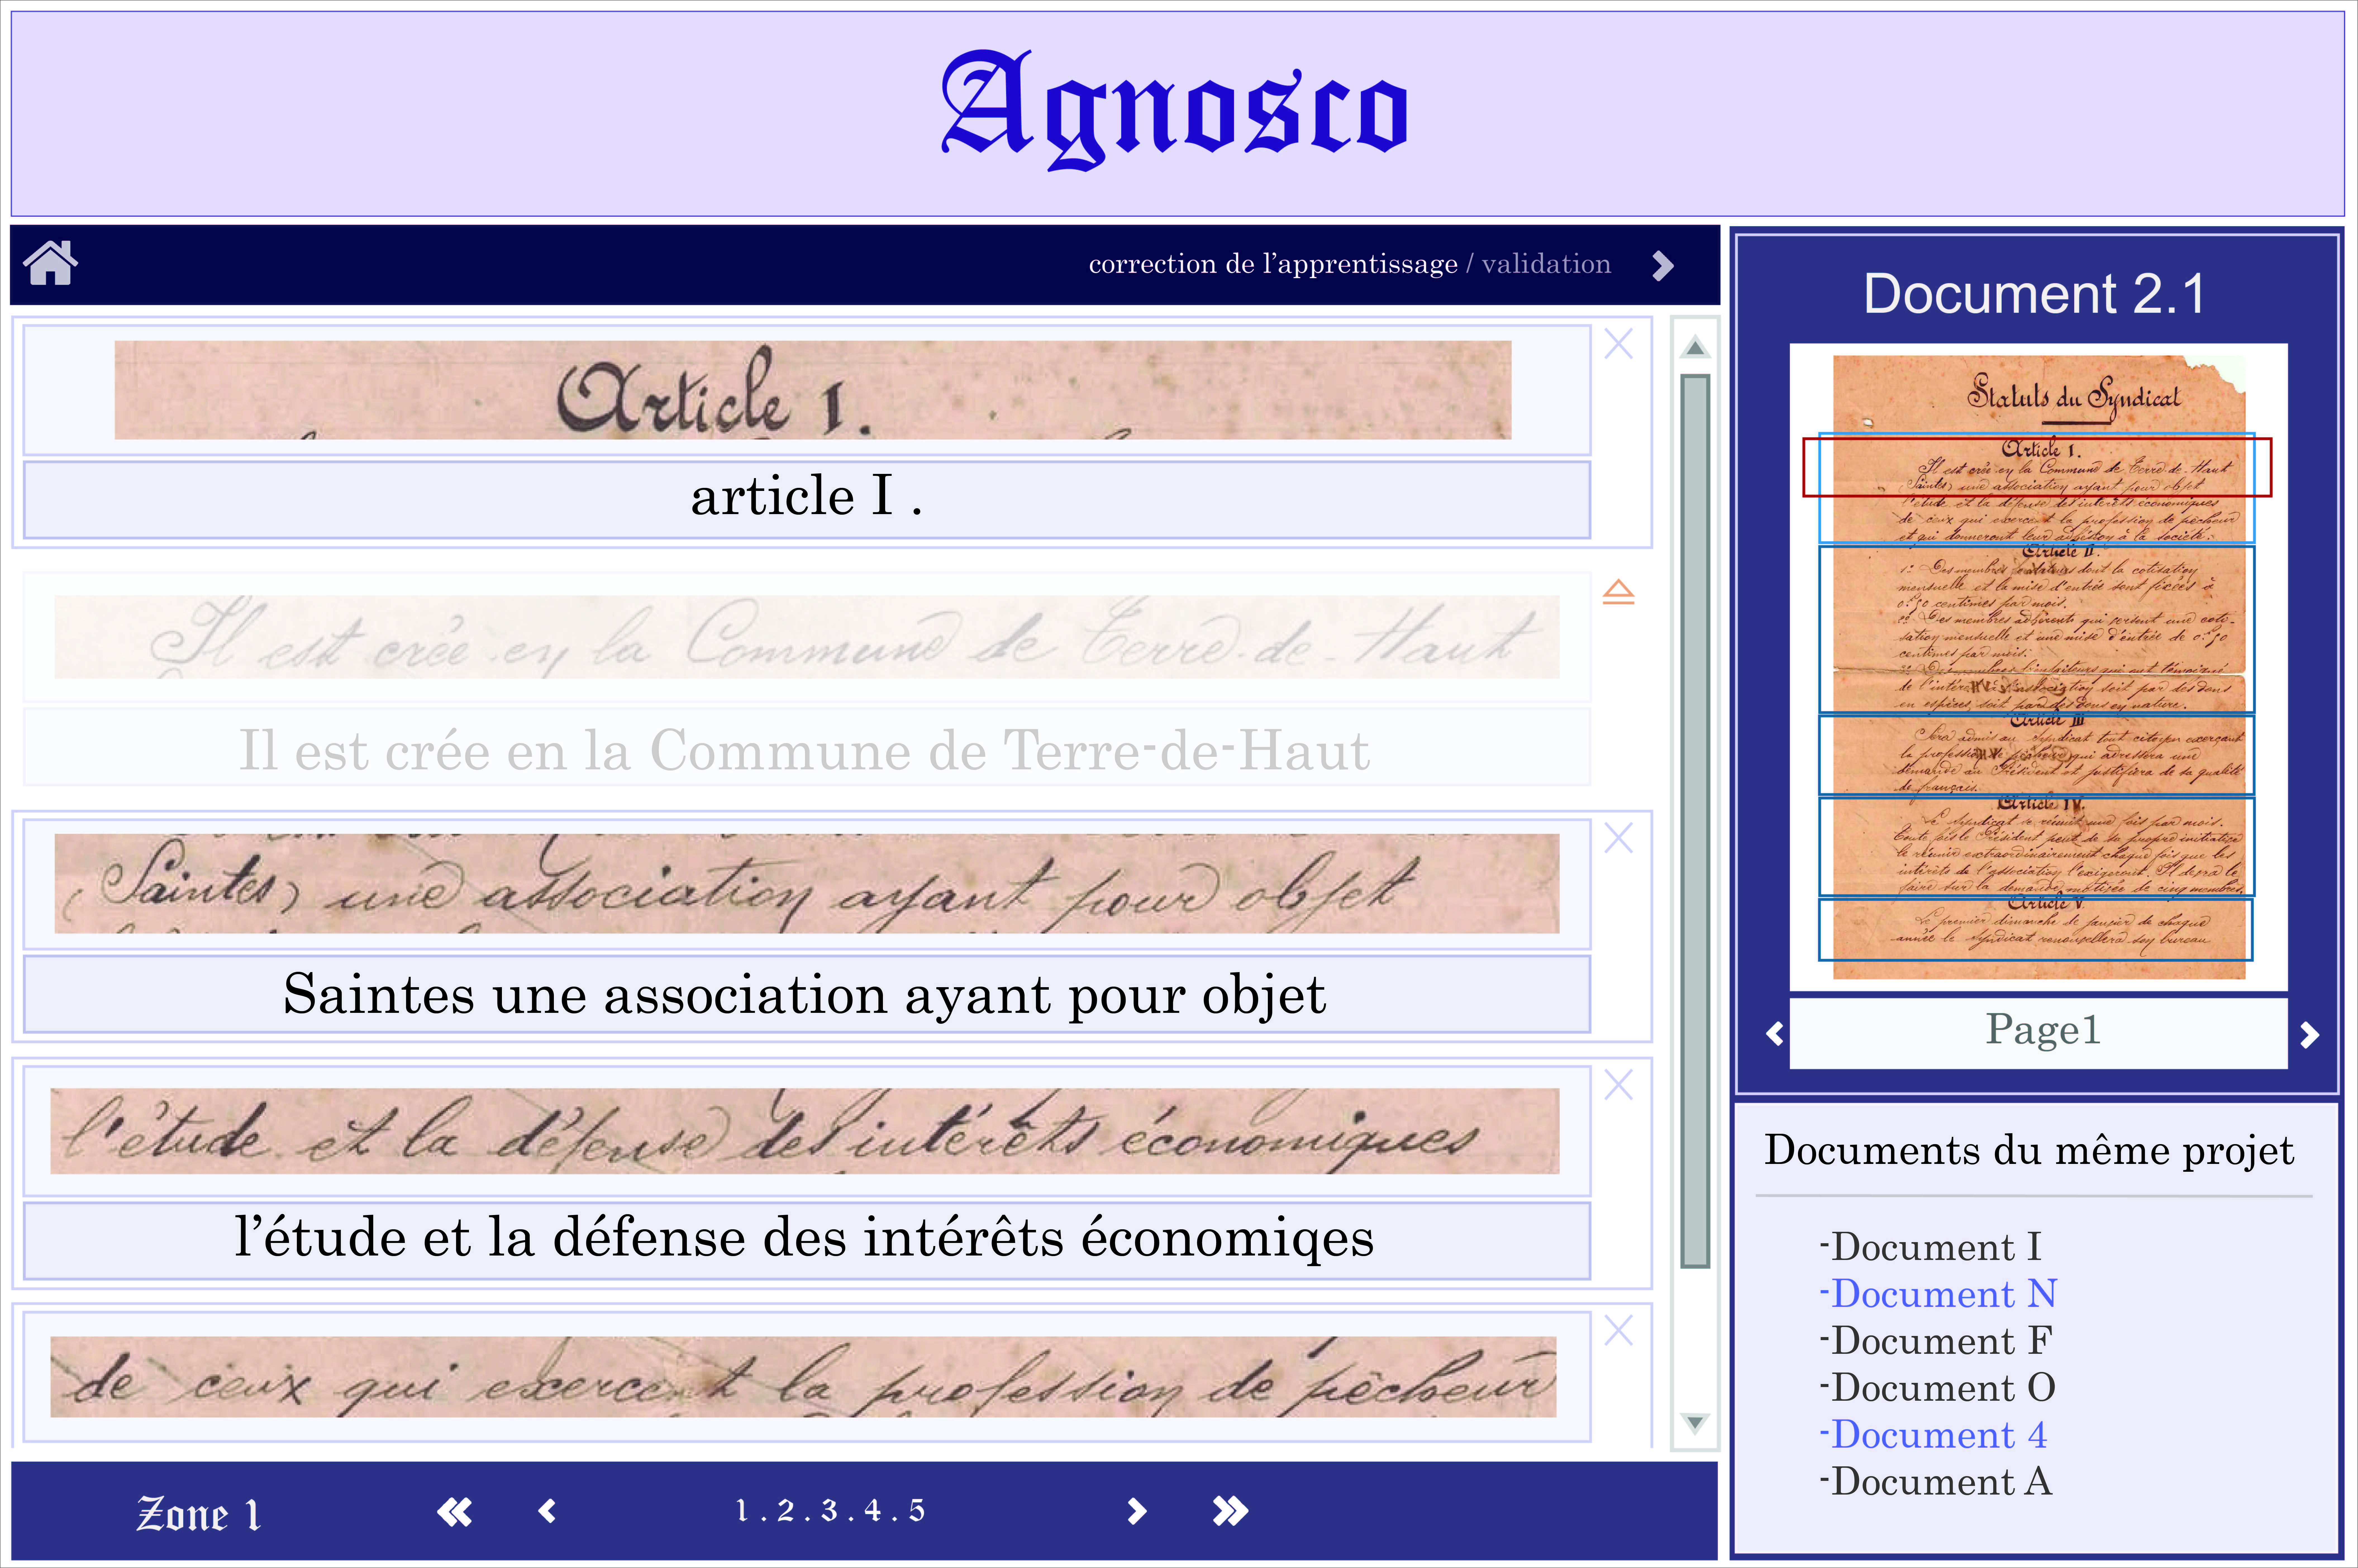
\includegraphics[scale=0.04]{assets/maquetteIHMcorrectionIA.jpg}
\end{center}
\end{mdframed}


\begin{mdframed}[frametitle={Figure 6 : Maquette de la page de validation finale lors de la deuxième itération}, innerbottommargin=10]
\begin{center}
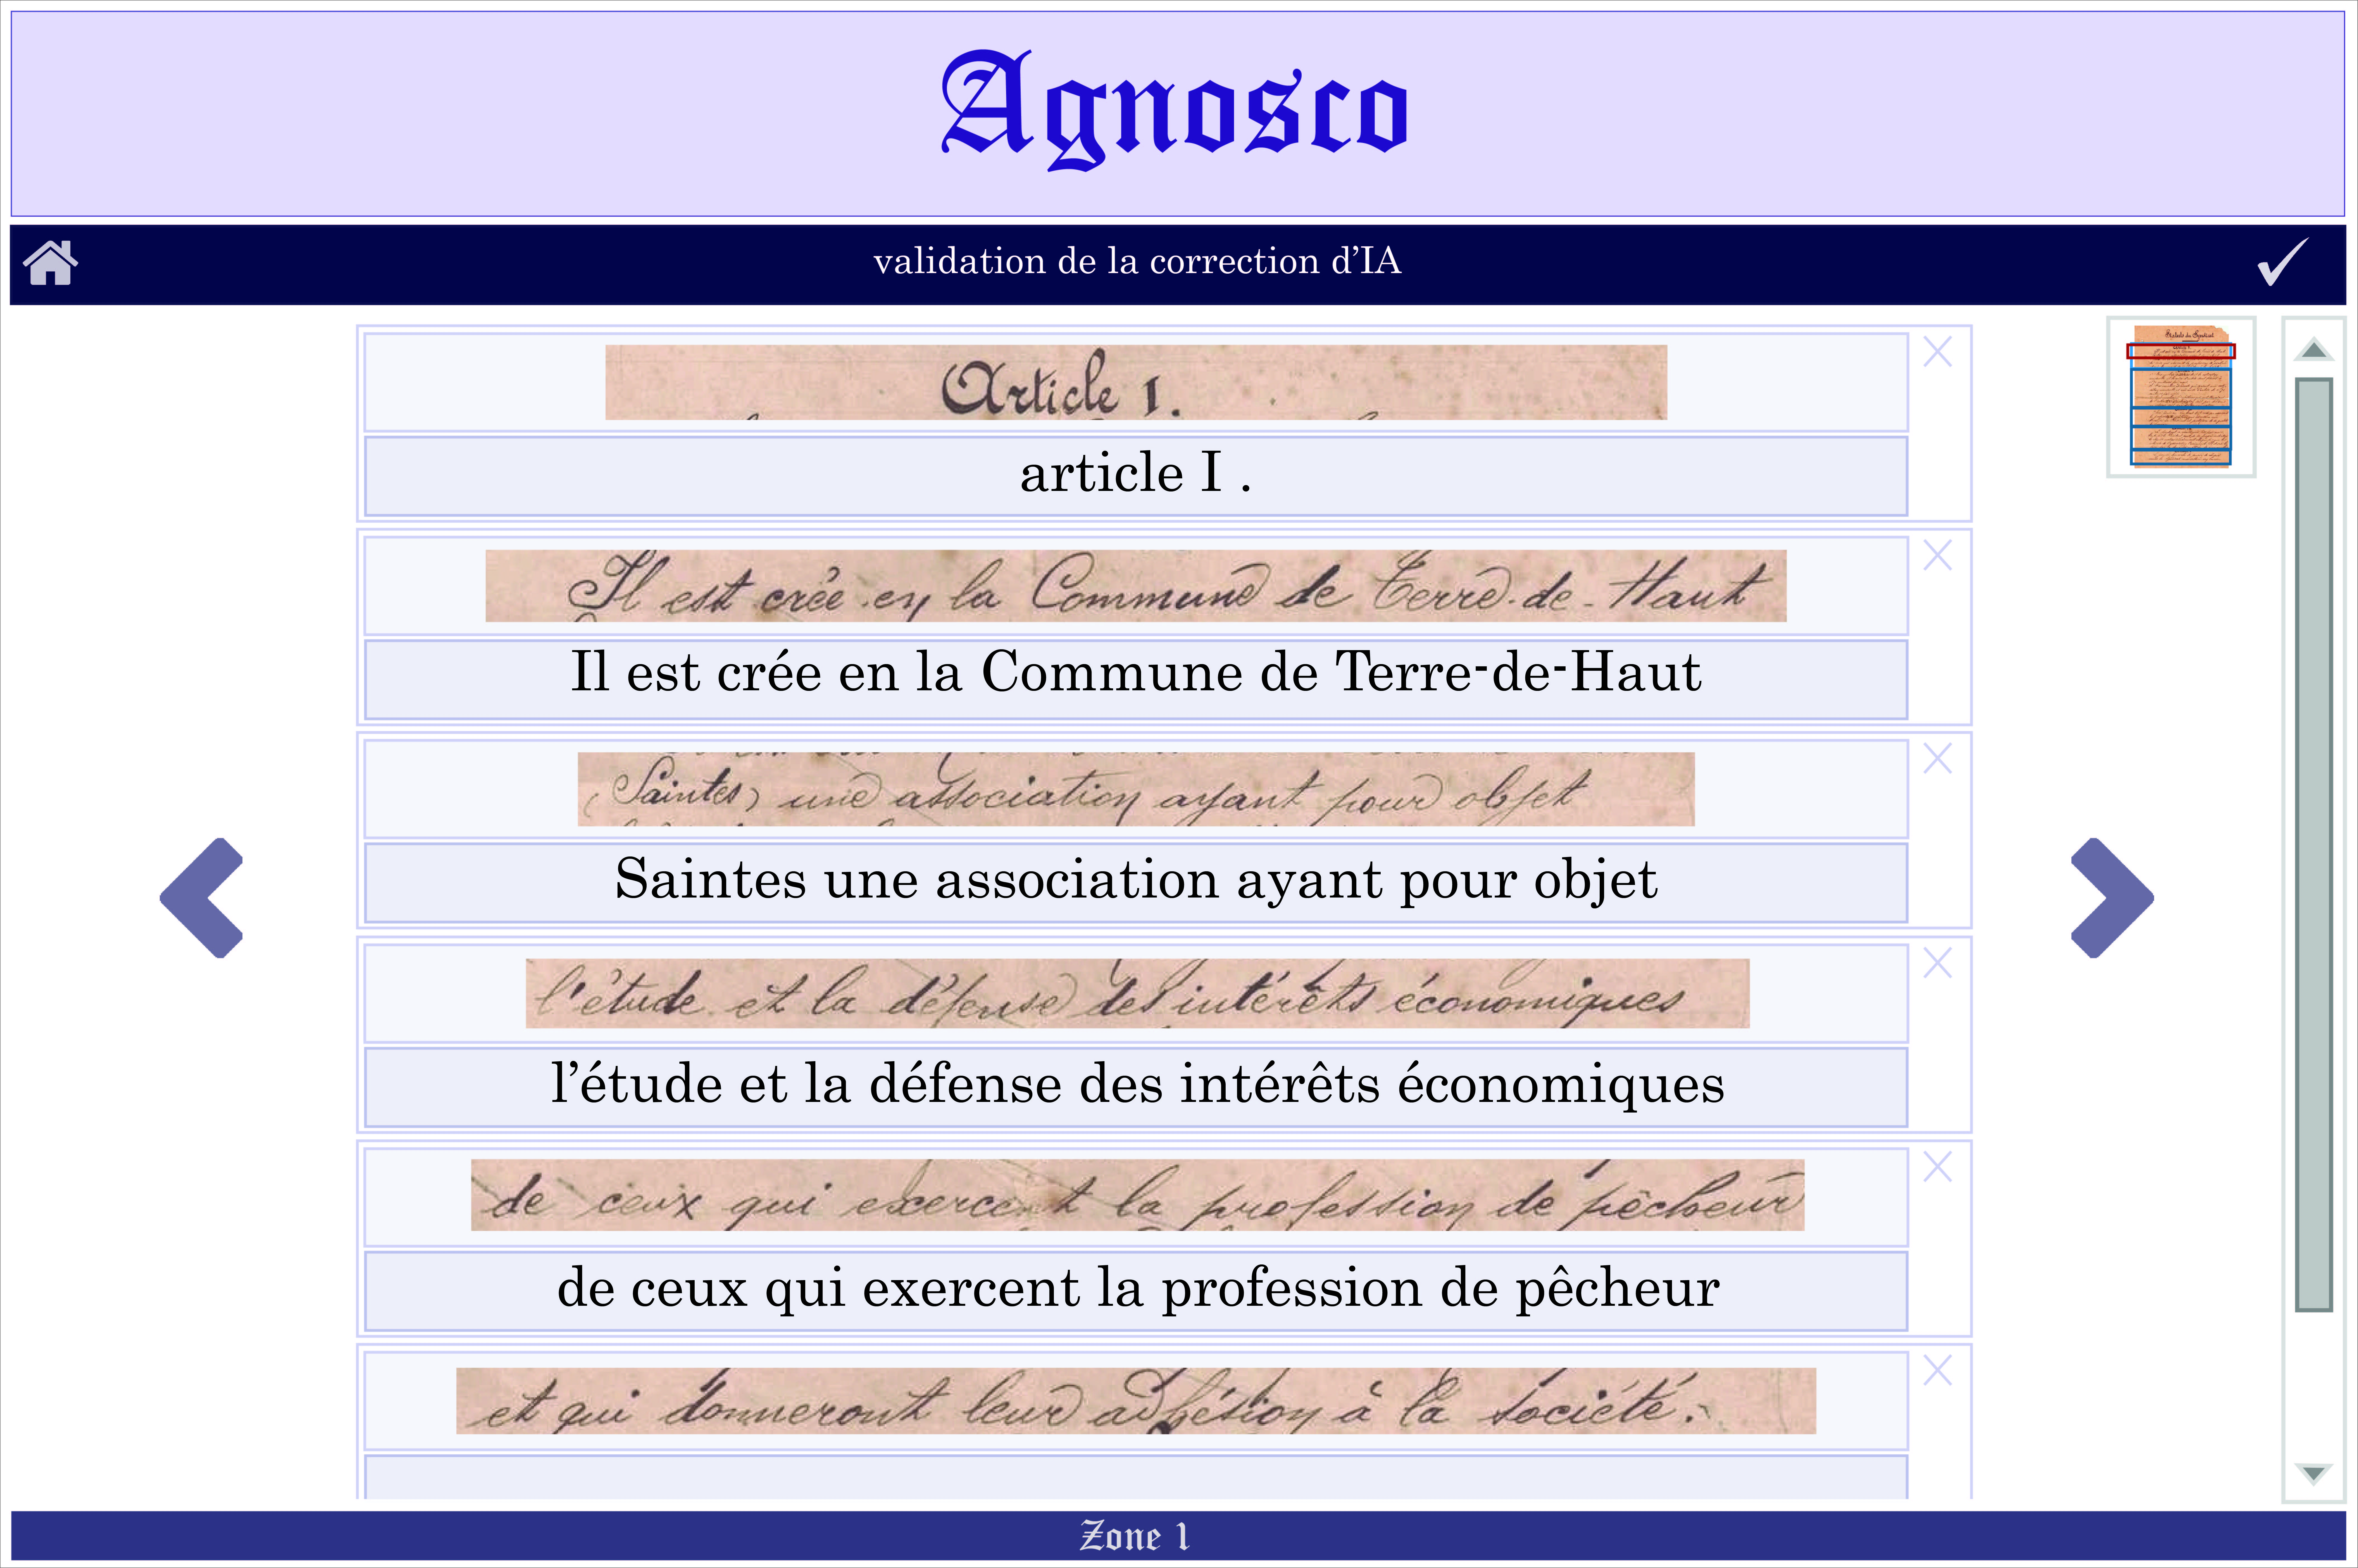
\includegraphics[scale=0.04]{assets/maquetteIHMvalidationIA.jpg}
\end{center}
\end{mdframed}